% Presentacion de defensa (Beamer) — version LaTeX del deck de sustentacion.
% Numeros = version corregida (post fix R1). Compilar: pdflatex beamer_defensa.tex
\documentclass[aspectratio=169,10pt]{beamer}
\usepackage[utf8]{inputenc}
\usepackage[T1]{fontenc}
\usepackage[spanish]{babel}
\usepackage{graphicx}
\usepackage{booktabs}
\usepackage{tikz}
\graphicspath{{../tesis_latex/}}

% ---------- paleta ----------
\definecolor{navy}{HTML}{15263D}
\definecolor{navylt}{HTML}{223A5E}
\definecolor{teal}{HTML}{1C7293}
\definecolor{amber}{HTML}{E9A23B}
\definecolor{seafoam}{HTML}{2A9D8F}
\definecolor{coral}{HTML}{D9534F}
\definecolor{ink}{HTML}{1B2733}
\definecolor{muted}{HTML}{63748A}
\definecolor{panel}{HTML}{EEF3F8}

% ---------- tema limpio (sin chrome) ----------
\usetheme{default}
\usefonttheme{professionalfonts}
\setbeamertemplate{navigation symbols}{}
\setbeamercolor{frametitle}{fg=navy}
\setbeamercolor{title}{fg=navy}
\setbeamercolor{structure}{fg=teal}
\setbeamercolor{normal text}{fg=ink}
\setbeamercolor{itemize item}{fg=amber}
\setbeamercolor{itemize subitem}{fg=teal}
\setbeamercolor{block title}{fg=white,bg=teal}
\setbeamercolor{block body}{fg=ink,bg=panel}
\setbeamercolor{block title alerted}{fg=white,bg=coral}
\setbeamercolor{block body alerted}{fg=ink,bg=panel}
\setbeamerfont{frametitle}{series=\bfseries,size=\large}
\setbeamerfont{title}{series=\bfseries}
\setbeamertemplate{itemize item}{\small\raise0.5pt\hbox{\textbullet}}
\setbeamertemplate{frametitle}{\vspace{4pt}\usebeamerfont{frametitle}\usebeamercolor[fg]{frametitle}\insertframetitle\par\vspace{-2pt}}
\setbeamertemplate{footline}{\hspace*{0.6cm}\textcolor{muted}{\tiny Estabilidad de XAI en GNNs para AML \textperiodcentered\ UTP 2026}\hfill\textcolor{muted}{\tiny\insertframenumber}\hspace*{0.6cm}\vspace{4pt}}

% helper: frame de seccion oscuro
\newcommand{\seccion}[1]{{%
\setbeamercolor{background canvas}{bg=navy}
\begin{frame}[plain]
\vfill
{\color{amber}\rule{0.9cm}{2pt}}\\[6pt]
{\color{white}\Large\bfseries #1}
\vfill
\end{frame}}}

\title{Estabilidad de Métodos de Explicabilidad (XAI) en Graph Neural Networks para la Detección de Lavado de Dinero bajo Desbalance Extremo}
\author{Alejandro Gómez Huertas \and Juan Diego Garzón Ovalle}
\institute{Director: Ph.D. Cristian Rosero Arias}
\date{Universidad Tecnológica de Pereira \textperiodcentered\ MISC \textperiodcentered\ 2026}

\begin{document}

% ===== 1. PORTADA =====
{\setbeamercolor{background canvas}{bg=navy}
\setbeamercolor{normal text}{fg=white}
\begin{frame}[plain]
\vspace{0.6cm}
{\color{amber}\footnotesize\bfseries UNIVERSIDAD TECNOLÓGICA DE PEREIRA \textperiodcentered\ MAESTRÍA EN INGENIERÍA EN SISTEMAS Y COMPUTACIÓN}\\[10pt]
{\color{white}\large\bfseries Estabilidad de Métodos de Explicabilidad (XAI)\\ en Graph Neural Networks para la Detección\\ de Lavado de Dinero bajo Desbalance Extremo}\\[10pt]
{\color{amber}\rule{1.2cm}{2pt}}\\[10pt]
{\color{white}\normalsize\bfseries Alejandro Gómez Huertas \quad\textperiodcentered\quad Juan Diego Garzón Ovalle}\\[4pt]
{\color{white!80}\small Director: Ph.D. Cristian Rosero Arias}\\[2pt]
{\color{white!80}\small Pereira, Colombia \textperiodcentered\ 2026}
\vfill
\end{frame}}

% ===== 2. AGENDA =====
\begin{frame}{Contenido}
\begin{enumerate}
  \item[\textcolor{teal}{\textbf{1}}] \textbf{Problema y motivación} — detección de lavado y la opacidad de las GNN
  \item[\textcolor{teal}{\textbf{2}}] \textbf{Pregunta y objetivos}
  \item[\textcolor{teal}{\textbf{3}}] \textbf{Metodología: dos ejes} — Elliptic real + grafo sintético con \textit{ground-truth}
  \item[\textcolor{teal}{\textbf{4}}] \textbf{Resultados} — estabilidad, plausibilidad, fidelidad y sus relaciones
  \item[\textcolor{teal}{\textbf{5}}] \textbf{Conclusiones} — aportes, límites y trabajo futuro
\end{enumerate}
\end{frame}

\seccion{1 \textperiodcentered\ Problema y motivación}

% ===== 3. EL PROBLEMA =====
\begin{frame}{El problema: detectar lavado sin caja negra}
\begin{columns}[T]
\begin{column}{0.56\textwidth}
\begin{itemize}
  \item El lavado mueve el \textbf{2--5\% del PIB mundial}; los sistemas por reglas generan \textbf{95--98\% de falsos positivos}.
  \item Las \textbf{GNN} modelan las transacciones como grafo y superan a lo tabular.
  \item \textbf{Pero son cajas negras}: en un entorno regulado, cada alerta debe ser justificable y reproducible.
\end{itemize}
\end{column}
\begin{column}{0.44\textwidth}
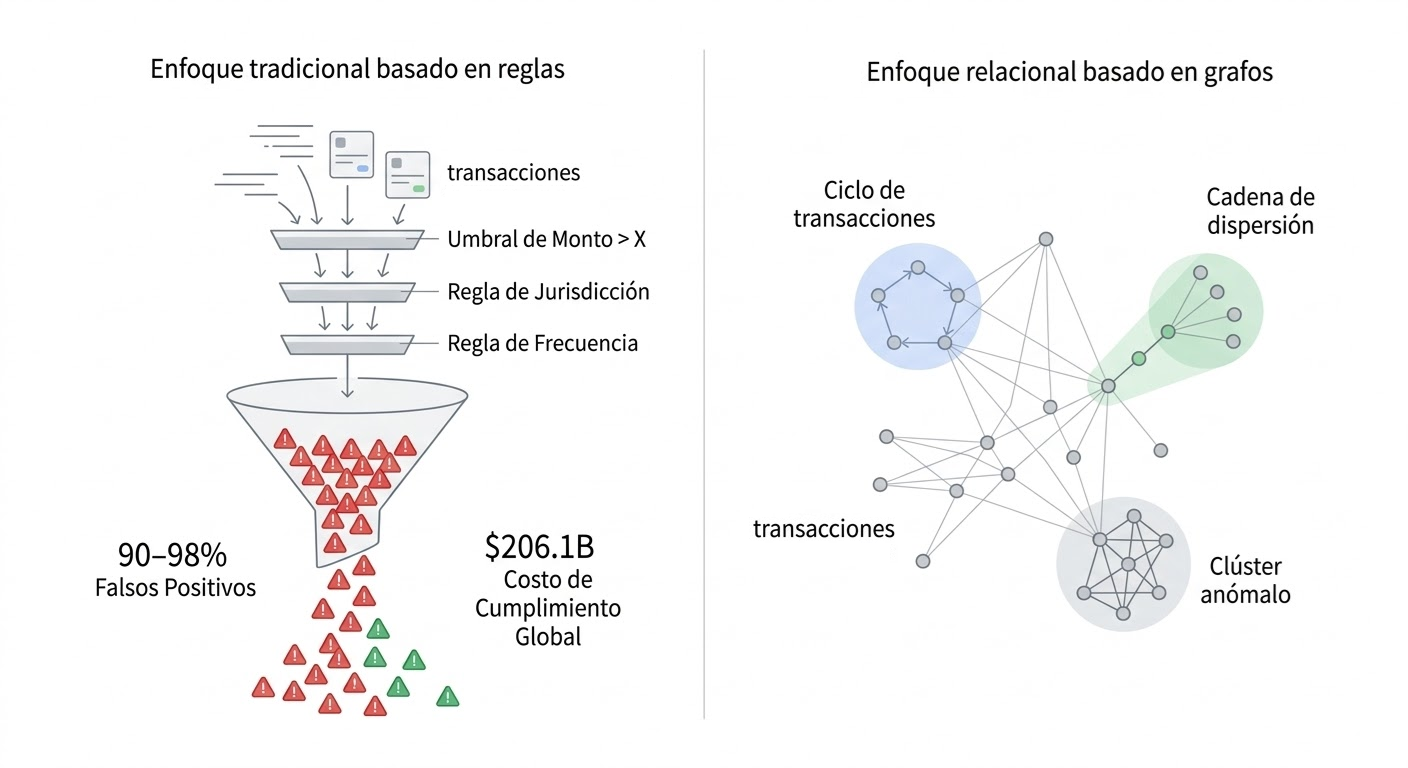
\includegraphics[width=\linewidth]{chapter_2/images_ch2/enfoques_moeny_laundering.png}
\end{column}
\end{columns}
\end{frame}

% ===== 4. PREGUNTA Y OBJETIVOS =====
\begin{frame}{Pregunta de investigación y objetivos}
\begin{block}{Pregunta}
¿Cómo se comporta la \textbf{estabilidad} de los métodos XAI sobre GNNs para AML bajo desbalance, y qué combinación de arquitectura, explicador y balanceo optimiza la interpretación robusta y auditable?
\end{block}
\vspace{3pt}
\begin{columns}[T]
\begin{column}{0.5\textwidth}
\begin{itemize}
  \item[\textcolor{amber}{\textbf{O1}}] Degradación de la estabilidad con el desbalance.
  \item[\textcolor{amber}{\textbf{O2}}] Resiliencia de GCN, GraphSAGE, GAT, TAGCN.
\end{itemize}
\end{column}
\begin{column}{0.5\textwidth}
\begin{itemize}
  \item[\textcolor{amber}{\textbf{O3}}] Impacto de las estrategias de balanceo.
  \item[\textcolor{amber}{\textbf{O4}}] Matriz de recomendación.
\end{itemize}
\end{column}
\end{columns}
\end{frame}

% ===== 5. LA BRECHA =====
\begin{frame}{La brecha en el estado del arte}
\begin{columns}[T]
\begin{column}{0.5\textwidth}
\begin{block}{Lo que ya se sabía}
\begin{itemize}\small
  \item Las GNN superan a lo tabular (Weber 2019).
  \item TAGCN + SHAP con alto rendimiento (He 2026).
  \item Predicción y explicabilidad, por separado.
\end{itemize}
\end{block}
\end{column}
\begin{column}{0.5\textwidth}
\begin{alertblock}{Lo que faltaba}
\begin{itemize}\small
  \item La \textbf{estabilidad} de las explicaciones sobre grafos AML no se había evaluado sistemáticamente.
  \item Elliptic no tiene \textit{ground-truth} de tipología $\Rightarrow$ la plausibilidad no era medible.
\end{itemize}
\end{alertblock}
\end{column}
\end{columns}
\end{frame}

\seccion{2 \textperiodcentered\ Marco conceptual}

% ===== 6. MARCO =====
\begin{frame}{Marco: redes de grafos y explicabilidad}
\begin{columns}[T]
\begin{column}{0.5\textwidth}
\textbf{\color{navy}4 arquitecturas GNN}
\begin{itemize}\small
  \item \textbf{GCN} — convolución espectral (1 salto)
  \item \textbf{GraphSAGE} — muestreo + agregación inductiva
  \item \textbf{GAT} — atención multi-cabeza
  \item \textbf{TAGCN} — filtros polinómicos de orden $K$
\end{itemize}
\end{column}
\begin{column}{0.5\textwidth}
\textbf{\color{navy}3 explicadores XAI (post-hoc)}
\begin{itemize}\small
  \item \textbf{GNNExplainer} — máscara por instancia
  \item \textbf{PGExplainer} — red generativa entrenada
  \item \textbf{GNNShap} — valores de Shapley por muestreo
\end{itemize}
\end{column}
\end{columns}
\end{frame}

% ===== 7. TRES PROPIEDADES =====
\begin{frame}{Tres propiedades que no son lo mismo}
\begin{columns}[T]
\begin{column}{0.33\textwidth}
\begin{block}{Estabilidad}\small ¿La explicación se reproduce entre semillas y perturbaciones?\end{block}
\end{column}
\begin{column}{0.33\textwidth}
\begin{block}{Plausibilidad}\small ¿Señala el patrón real de lavado (\textit{ground-truth})?\end{block}
\end{column}
\begin{column}{0.33\textwidth}
\begin{block}{Fidelidad}\small ¿Refleja de verdad la decisión interna del modelo?\end{block}
\end{column}
\end{columns}
\vspace{8pt}
\begin{center}
\textcolor{amber}{\textbf{Tesis central:}} \textit{las tres son empíricamente independientes.}
\end{center}
\end{frame}

\seccion{3 \textperiodcentered\ Metodología}

% ===== 8. DOS EJES =====
\begin{frame}{Metodología: un diseño de dos ejes}
\begin{columns}[T]
\begin{column}{0.5\textwidth}
\begin{block}{Eje 1 \textperiodcentered\ Elliptic (real)}
\begin{itemize}\small
  \item Validez \textbf{externa}: transacciones reales.
  \item Sin \textit{ground-truth} $\Rightarrow$ solo estabilidad.
  \item Campo receptivo minúsculo ($\sim$2 nodos).
\end{itemize}
\end{block}
\end{column}
\begin{column}{0.5\textwidth}
\begin{block}{Eje 2 \textperiodcentered\ Sintético (propio)}
\begin{itemize}\small
  \item Validez \textbf{interna}: \textit{ground-truth} por nodo y arista.
  \item Permite medir plausibilidad y fidelidad.
  \item 4 tipologías estándar; 3 realizaciones.
\end{itemize}
\end{block}
\end{column}
\end{columns}
\end{frame}

% ===== 9. DISENO FACTORIAL =====
\begin{frame}{Diseño factorial}
\begin{center}
{\color{teal}\Large\textbf{4}} arquitecturas \; $\times$ \; {\color{amber}\Large\textbf{3}} explicadores \; $\times$ \; {\color{seafoam}\Large\textbf{3}} balanceos \; $\times$ \; {\color{coral}\Large\textbf{5}} escenarios
\end{center}
\vspace{2pt}
\begin{center}\small = 60 configuraciones por eje \, $\times$ 3 explicadores para el estudio de estabilidad\end{center}
\vspace{4pt}
\begin{block}{Protocolo de robustez}
\small Estabilidad: 5 réplicas estocásticas por explicación. Inferencia (eje sintético): 3 semillas de modelo $\times$ 3 grafos, con Kruskal-Wallis, Wilcoxon e IC bootstrap.
\end{block}
\end{frame}

% ===== 10. ELLIPTIC =====
\begin{frame}{Eje 1 — Elliptic Bitcoin Dataset}
\begin{columns}[T]
\begin{column}{0.54\textwidth}
\begin{itemize}\small
  \item 203.769 nodos \textperiodcentered\ 234.355 aristas \textperiodcentered\ 166 features \textperiodcentered\ 49 pasos.
  \item Ilícitas $\sim$2,2\% (razón $\sim$1:9 en el subconjunto etiquetado).
  \item Split temporal causal (train 1--34 / val 35--42 / test 43--49).
  \item Campo receptivo mediana $\sim$2 nodos $\Rightarrow$ solo el Spearman discrimina.
\end{itemize}
\end{column}
\begin{column}{0.46\textwidth}
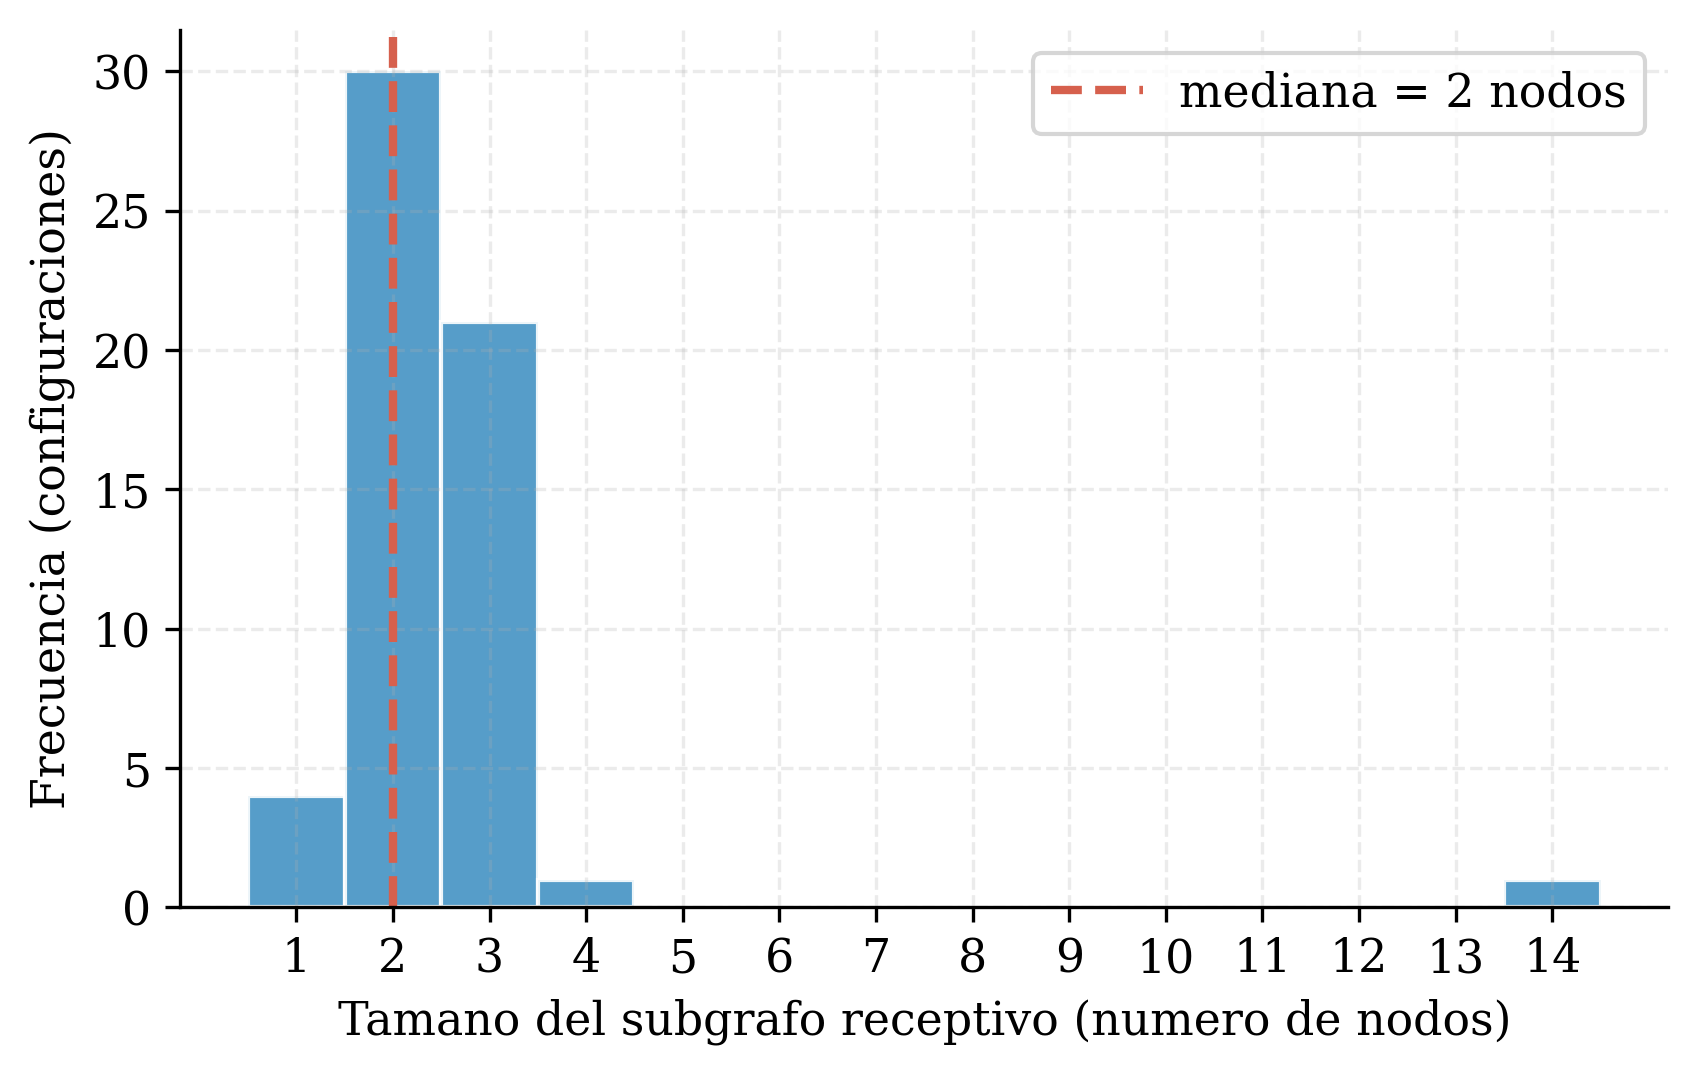
\includegraphics[width=\linewidth]{chapter_4/images_ch4/dispersion_elliptic.png}
\end{column}
\end{columns}
\end{frame}

% ===== 11. SINTETICO =====
\begin{frame}{Eje 2 — grafo sintético con ground-truth}
\begin{columns}[T]
\begin{column}{0.54\textwidth}
\begin{itemize}\small
  \item \textbf{¿Por qué?} medir plausibilidad exige saber cuál subgrafo es el patrón — Elliptic no lo da.
  \item 4 tipologías: \textit{structuring}, \textit{layering}, \textit{fan-in}, \textit{fan-out}.
  \item Aristas distractoras + firma atenuada $\Rightarrow$ la métrica discrimina.
  \item \textit{Ground-truth} ciego al explicador; 3 realizaciones.
\end{itemize}
\end{column}
\begin{column}{0.46\textwidth}
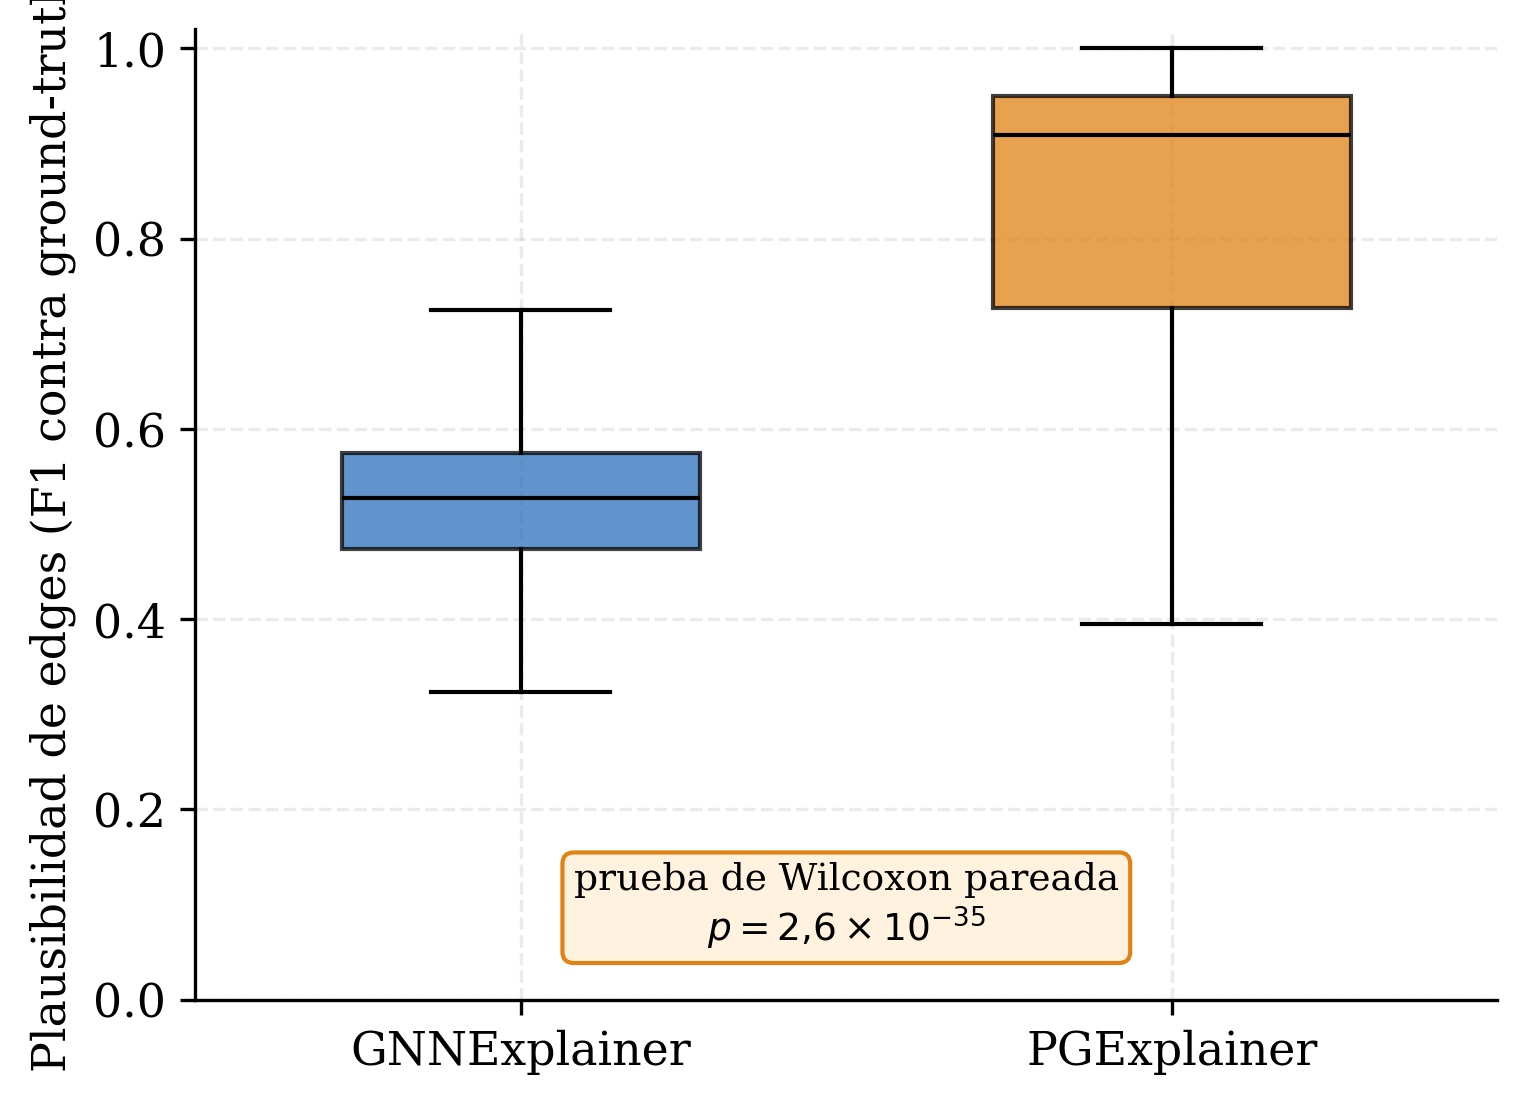
\includegraphics[width=\linewidth]{chapter_5/images_ch5/hallazgo_estrella.png}
\end{column}
\end{columns}
\end{frame}

% ===== 12. METRICAS =====
\begin{frame}{Métricas y protocolo estadístico}
\begin{itemize}
  \item \textbf{\color{teal}Estabilidad} — correlación de Spearman entre rankings de features (primaria).
  \item \textbf{\color{seafoam}Plausibilidad} — coincidencia con el \textit{ground-truth} de la tipología.
  \item \textbf{\color{amber}Fidelidad} — caída de la predicción al retirar lo importante.
  \item \textbf{\color{coral}Rendimiento} — PR-AUC como métrica primaria (el F1 en umbral es degenerado bajo desbalance).
\end{itemize}
\vspace{3pt}
\small Estadística: Kruskal-Wallis, Wilcoxon, intervalos de confianza \textit{bootstrap}.
\end{frame}

\seccion{4 \textperiodcentered\ Resultados}

% ===== 13. DOS ARTEFACTOS =====
\begin{frame}{Contribución: dos artefactos de evaluación}
\begin{columns}[T]
\begin{column}{0.5\textwidth}
\begin{alertblock}{1 \textperiodcentered\ Fallo de memoria silencioso}
\small Cálculo sobre el grafo completo $\Rightarrow$ 13 configuraciones de GAT fallaban en silencio $\Rightarrow$ favorecía a GAT.
\end{alertblock}
\end{column}
\begin{column}{0.5\textwidth}
\begin{alertblock}{2 \textperiodcentered\ Truncamiento del Spearman}
\small La métrica descartaba features fuera del umbral $\Rightarrow$ rankings mutilados $\Rightarrow$ favorecía a GraphSAGE.
\end{alertblock}
\end{column}
\end{columns}
\vspace{5pt}
\begin{center}\small
\textcolor{navy}{\textbf{Cada uno bastaba para una conclusión comparativa falsa.}} La estabilidad depende del protocolo de medición.\\ Además: dos \textit{bugs} reportables en el PGExplainer de PyG 2.7.
\end{center}
\end{frame}

% ===== 14. RANKING =====
\begin{frame}{Resultado 1 — estabilidad por arquitectura}
\begin{columns}[T]
\begin{column}{0.5\textwidth}
\begin{itemize}\small
  \item[\textcolor{teal}{$\blacksquare$}] \textbf{GAT} \hfill 0,780
  \item[\textcolor{teal}{$\blacksquare$}] \textbf{GCN} \hfill 0,778
  \item[\textcolor{seafoam}{$\blacksquare$}] GraphSAGE \hfill 0,735
  \item[\textcolor{muted}{$\blacksquare$}] TAGCN \hfill 0,580
\end{itemize}
\vspace{4pt}
\small \textbf{GAT y GCN lideran} (ya no GraphSAGE, que era artefacto). GAT vs GraphSAGE: \textit{no significativo} (Wilcoxon $p=0{,}375$).
\end{column}
\begin{column}{0.5\textwidth}
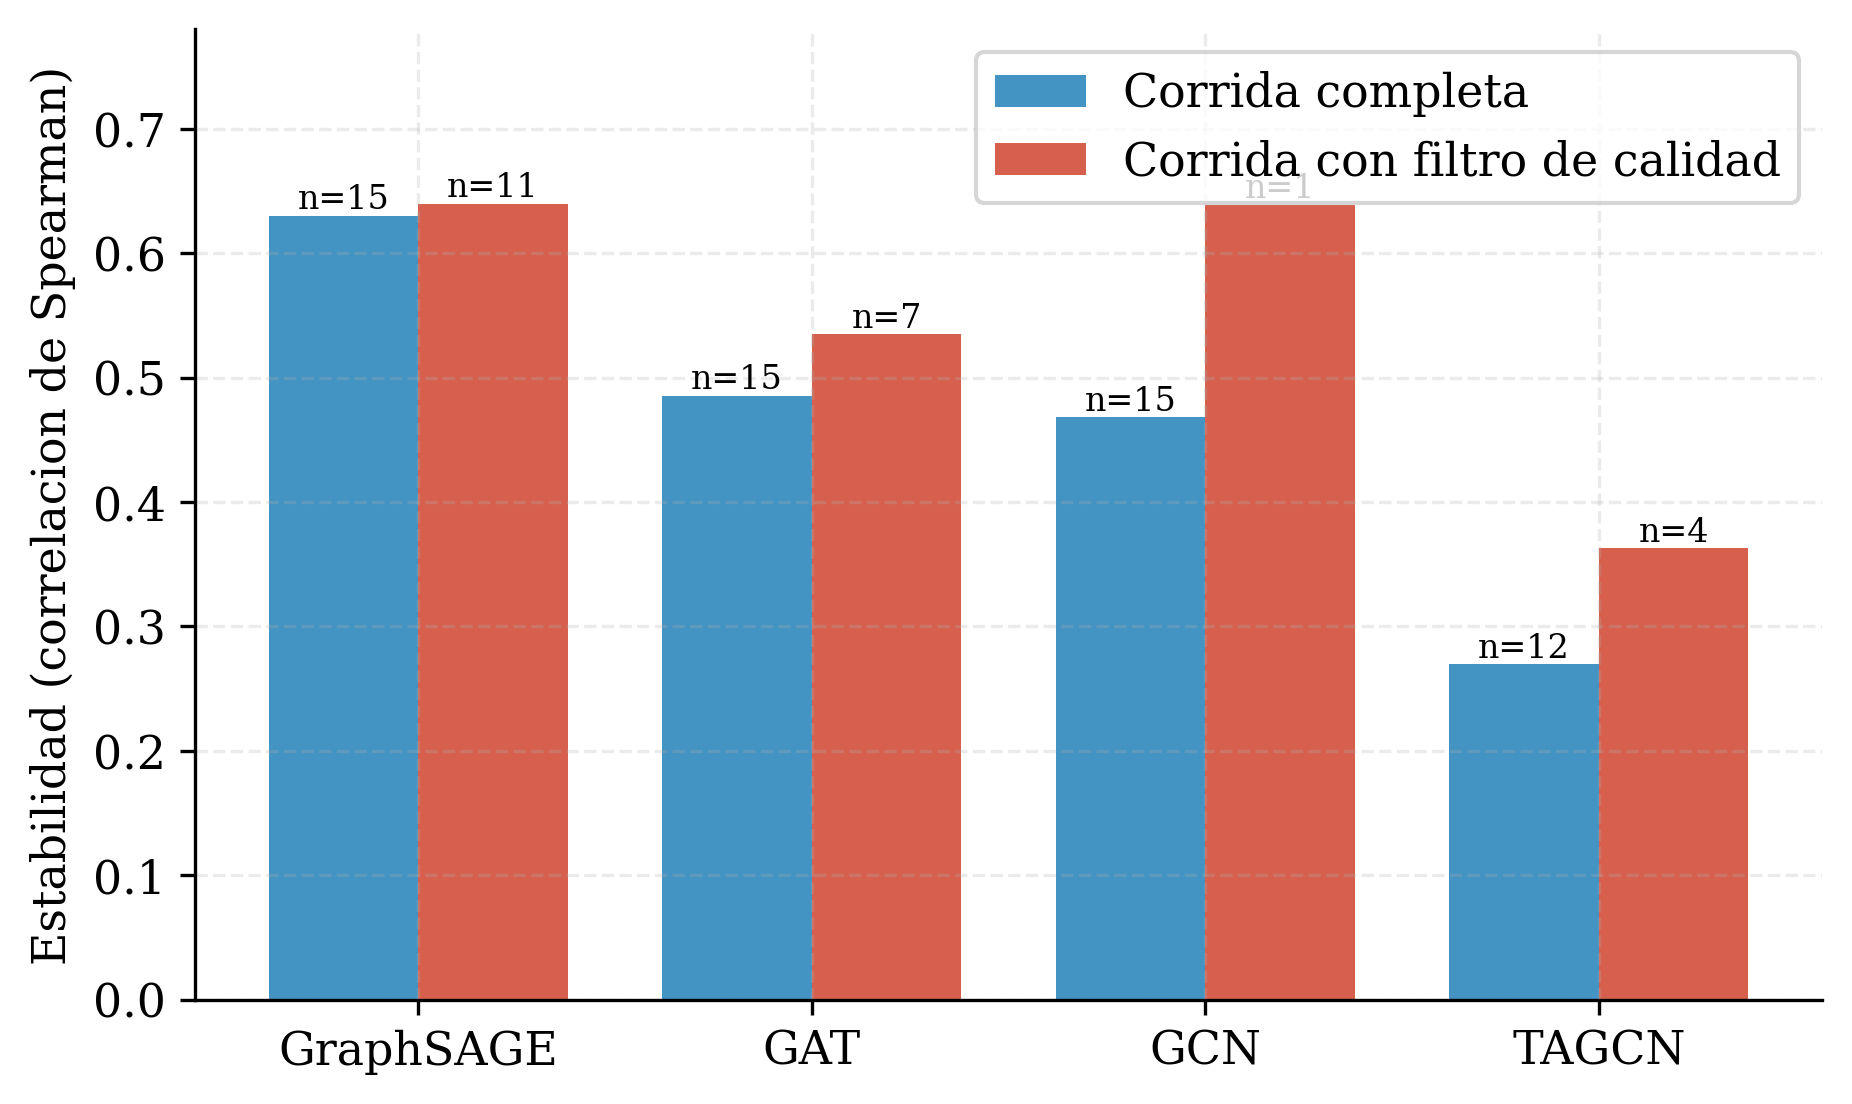
\includegraphics[width=\linewidth]{chapter_4/images_ch4/ranking_khop.png}
\end{column}
\end{columns}
\end{frame}

% ===== 15. CONCORDANCIA =====
\begin{frame}{Resultado 1b — concordancia entre regímenes}
\begin{columns}[T]
\begin{column}{0.5\textwidth}
\begin{itemize}\small
  \item La ``inversión por densidad'' era un \textbf{artefacto} de la métrica.
  \item Corregida, Elliptic (disperso) \textbf{concuerda} con el sintético (denso).
\end{itemize}
\vspace{6pt}
\begin{center}
\small Correlación de rangos entre regímenes\\[4pt]
{\color{coral}\Large\textbf{$-0{,}20$}} \; $\rightarrow$ \; {\color{amber}\Large\textbf{$+0{,}80$}}\\[2pt]
{\footnotesize métrica con bug \; $\rightarrow$ \; métrica corregida}
\end{center}
\end{column}
\begin{column}{0.5\textwidth}
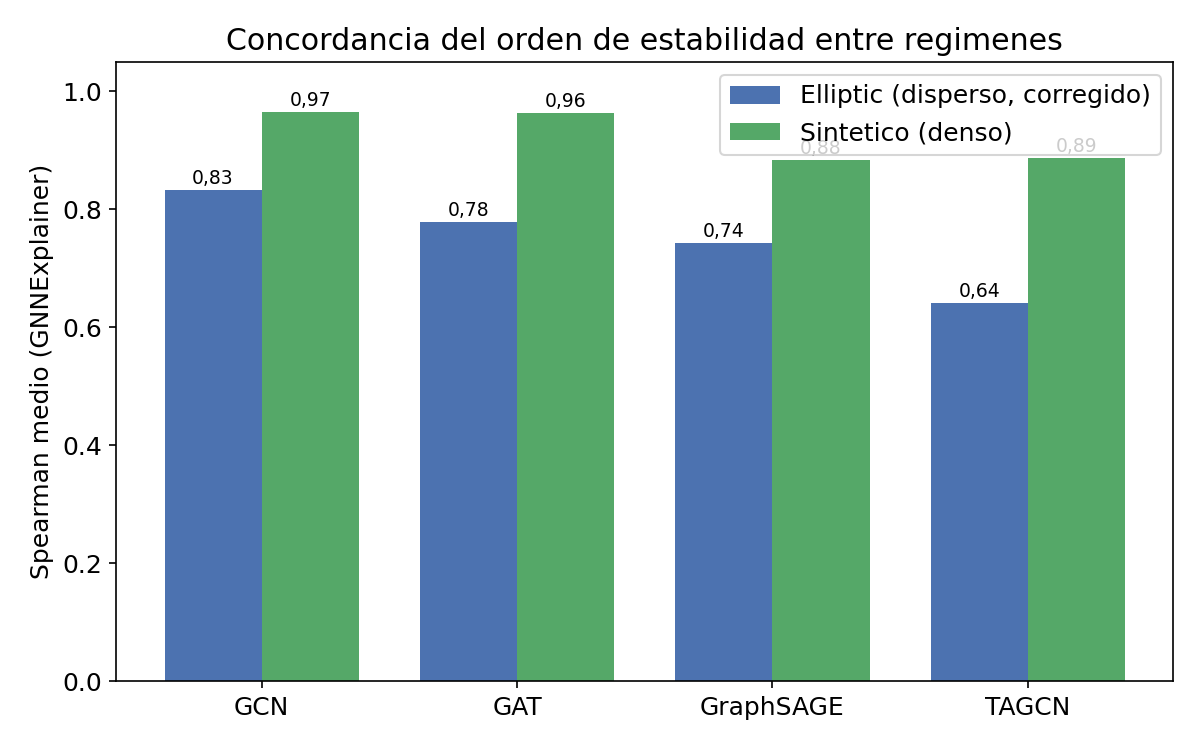
\includegraphics[width=\linewidth]{chapter_5/images_ch5/contraste_regimen.png}
\end{column}
\end{columns}
\end{frame}

% ===== 16. DISOCIACION =====
\begin{frame}{Resultado 2 — disociación plausibilidad / fidelidad}
\begin{columns}[T]
\begin{column}{0.52\textwidth}
\begin{itemize}\small
  \item \textbf{\color{teal}PGExplainer} recupera mejor el patrón: plausibilidad 0,80 vs 0,50 (Wilcoxon $p\approx 2{,}6\times10^{-35}$)\dots
  \item \dots pero \textbf{\color{coral}colapsa en fidelidad}: 0,11 vs 0,56 de GNNExplainer.
  \item \textit{El explicador más ``plausible'' no es el más fiel.}
\end{itemize}
\end{column}
\begin{column}{0.48\textwidth}
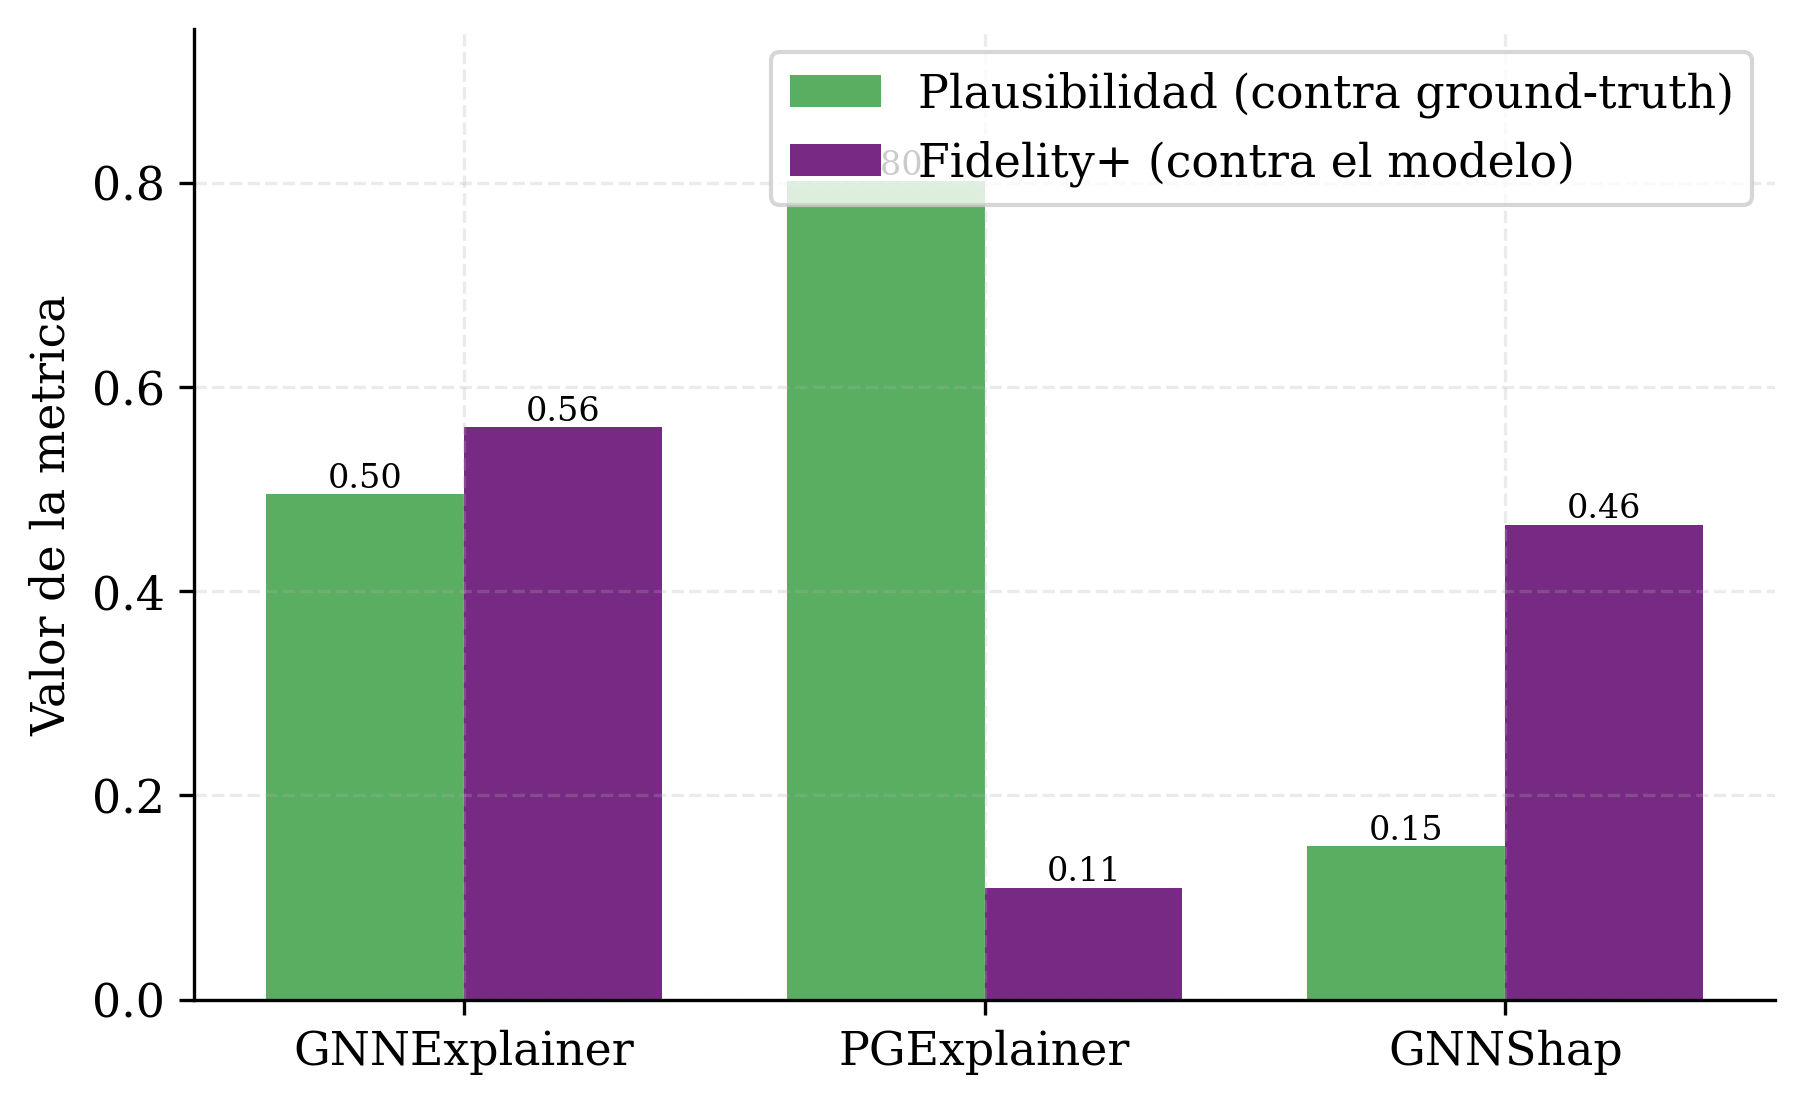
\includegraphics[width=\linewidth]{chapter_5/images_ch5/disociacion.png}
\end{column}
\end{columns}
\end{frame}

% ===== 17. PUENTE NULO =====
\begin{frame}{Resultado 3 — puente nulo y balanceo irrelevante}
\begin{columns}[T]
\begin{column}{0.52\textwidth}
\begin{itemize}\small
  \item Hipótesis central (estable $\Rightarrow$ plausible): \textbf{\color{coral}refutada}.
  \item Correlación estabilidad--plausibilidad $r=-0{,}01$ (IC 95\% incluye el cero).
  \item El balanceo es prácticamente \textbf{irrelevante} ($\eta^2 < 0{,}02$).
  \item \textit{Un no-resultado, reportado con honestidad.}
\end{itemize}
\end{column}
\begin{column}{0.48\textwidth}
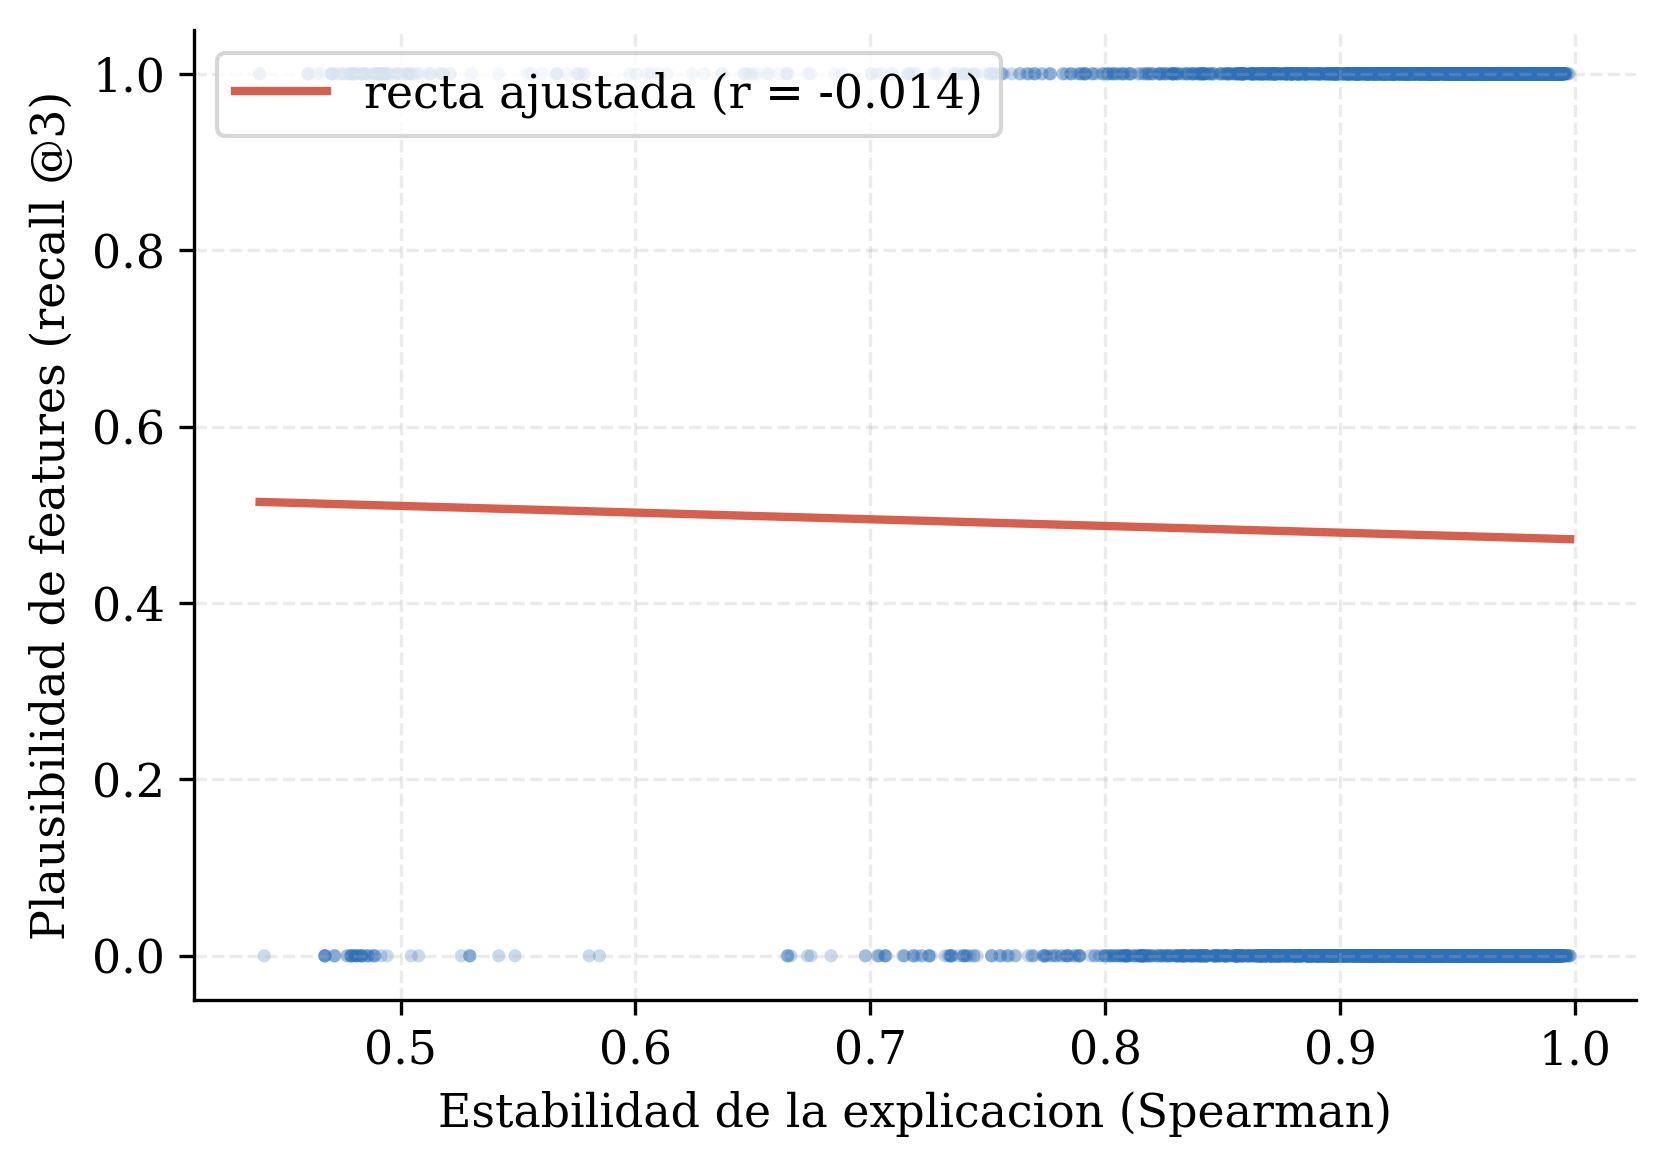
\includegraphics[width=\linewidth]{chapter_5/images_ch5/puente_nulo.png}
\end{column}
\end{columns}
\end{frame}

% ===== 18. COLAPSO VAL->TEST =====
\begin{frame}{Rendimiento y colapso validación $\rightarrow$ test}
\begin{columns}[T]
\begin{column}{0.33\textwidth}
\begin{block}{PR-AUC}\centering 0,367 \\ {\footnotesize\color{muted}validación}\\ $\rightarrow$ test \textbf{\color{coral}0,017}\end{block}
\end{column}
\begin{column}{0.33\textwidth}
\begin{block}{ROC-AUC}\centering 0,884 \\ {\footnotesize\color{muted}validación}\\ $\rightarrow$ test \textbf{\color{coral}0,653}\end{block}
\end{column}
\begin{column}{0.33\textwidth}
\begin{block}{Precision@50}\centering 0,657 \\ {\footnotesize\color{muted}validación}\\ $\rightarrow$ test \textbf{\color{coral}0,020}\end{block}
\end{column}
\end{columns}
\vspace{6pt}
\begin{center}\small
El \textbf{ROC-AUC es engañoso} bajo desbalance $\Rightarrow$ PR-AUC y precision@k como primarias.\\
La estabilidad se estudia sobre verdaderos positivos de \textbf{validación} (encuadre declarado).
\end{center}
\end{frame}

\seccion{5 \textperiodcentered\ Conclusiones}

% ===== 19. MATRIZ DE RECOMENDACION =====
\begin{frame}{Matriz de recomendación}
\begin{center}
\renewcommand{\arraystretch}{1.5}
\begin{tabular}{ll}
\toprule
\textbf{Objetivo operativo} & \textbf{Configuración} \\
\midrule
Auditabilidad / estabilidad & \textcolor{teal}{\textbf{GAT} o \textbf{GCN}} \\
Recuperar el patrón (plausibilidad) & \textcolor{seafoam}{\textbf{PGExplainer}} \\
Fidelidad al modelo & \textcolor{amber}{\textbf{GNNExplainer}} \\
Estabilidad interna del método & \textcolor{coral}{\textbf{GNNShap}} \\
\bottomrule
\end{tabular}
\end{center}
\end{frame}

% ===== 20. CONTRIBUCIONES / LIMITES =====
\begin{frame}{Contribuciones y limitaciones}
\begin{columns}[T]
\begin{column}{0.5\textwidth}
\begin{block}{Contribuciones}
\begin{itemize}\small
  \item Tres dimensiones independientes.
  \item Corrección de dos artefactos + dos \textit{bugs} de PGExplainer.
  \item Generador sintético con \textit{ground-truth} por arista.
  \item Matriz de recomendación.
\end{itemize}
\end{block}
\end{column}
\begin{column}{0.5\textwidth}
\begin{alertblock}{Limitaciones (declaradas)}
\begin{itemize}\small
  \item La inferencia fuerte proviene del eje sintético.
  \item El clasificador colapsa en test (\textit{shift} temporal).
  \item Una sola semilla de modelo en Elliptic.
\end{itemize}
\end{alertblock}
\end{column}
\end{columns}
\end{frame}

% ===== 21. CONCLUSIONES / CIERRE =====
{\setbeamercolor{background canvas}{bg=navy}
\setbeamercolor{normal text}{fg=white}
\begin{frame}[plain]
\vspace{0.3cm}\par
{\color{amber}\rule{0.9cm}{2pt}}\par\vspace{6pt}
{\color{white}\large\bfseries Conclusiones}\par\vspace{8pt}
{\color{white}\small
\begin{itemize}
  \item Estabilidad $\neq$ plausibilidad $\neq$ fidelidad: el mejor explicador depende del objetivo.
  \item Con la medición corregida, datos reales y sintéticos cuentan una historia coherente (GAT/GCN estables).
  \item La estabilidad de una explicación depende del protocolo de evaluación, no solo del método.
\end{itemize}}
\vspace{4pt}\par
{\color{white!85}\small \textbf{Trabajo futuro:} Elliptic2, AMLSim, GNNs temporales, GraphSMOTE.}\par\vspace{12pt}
\begin{center}
{\color{white}\Large\bfseries Gracias \textperiodcentered\ Preguntas}\par\vspace{2pt}
{\color{white!80}\small Alejandro Gómez Huertas \textperiodcentered\ Juan Diego Garzón Ovalle}
\end{center}
\end{frame}}

\end{document}
